%! TEX root = ./master.tex

\lecture{24}{Week: 11}{Non-Uniform Memory Access(NUMA)}

\subsubsection{Non-Uniform Memory Access (NUMA)}
\paragraph{SMP Limitations}
SMP is not well suited for scalability. While we may add more cache to compensate for adding more cores, the main bottleneck is the memory bandwidth. Using a memory bus, only one CPU can communicate via the bus at the time. NUMB arises due to theses limitations. In this architecture, the memory bus is replaced by a interconnection network.

NUMA is pretty common in modern systems (mainly servers).

\paragraph{Distributed Memory Architecture}
There are multiple slices, each containing one or multiple CPU cores, own ram and directory and a interconnection part to other slices. Adding more CPUs (more slices) brings more of most other things too (RAM etc.). This allows for scalability to 1000s of cores. The interconnects are not buses but it is network like. It carries messages between nodes like read/write requests/responses, cache invalidates etc.

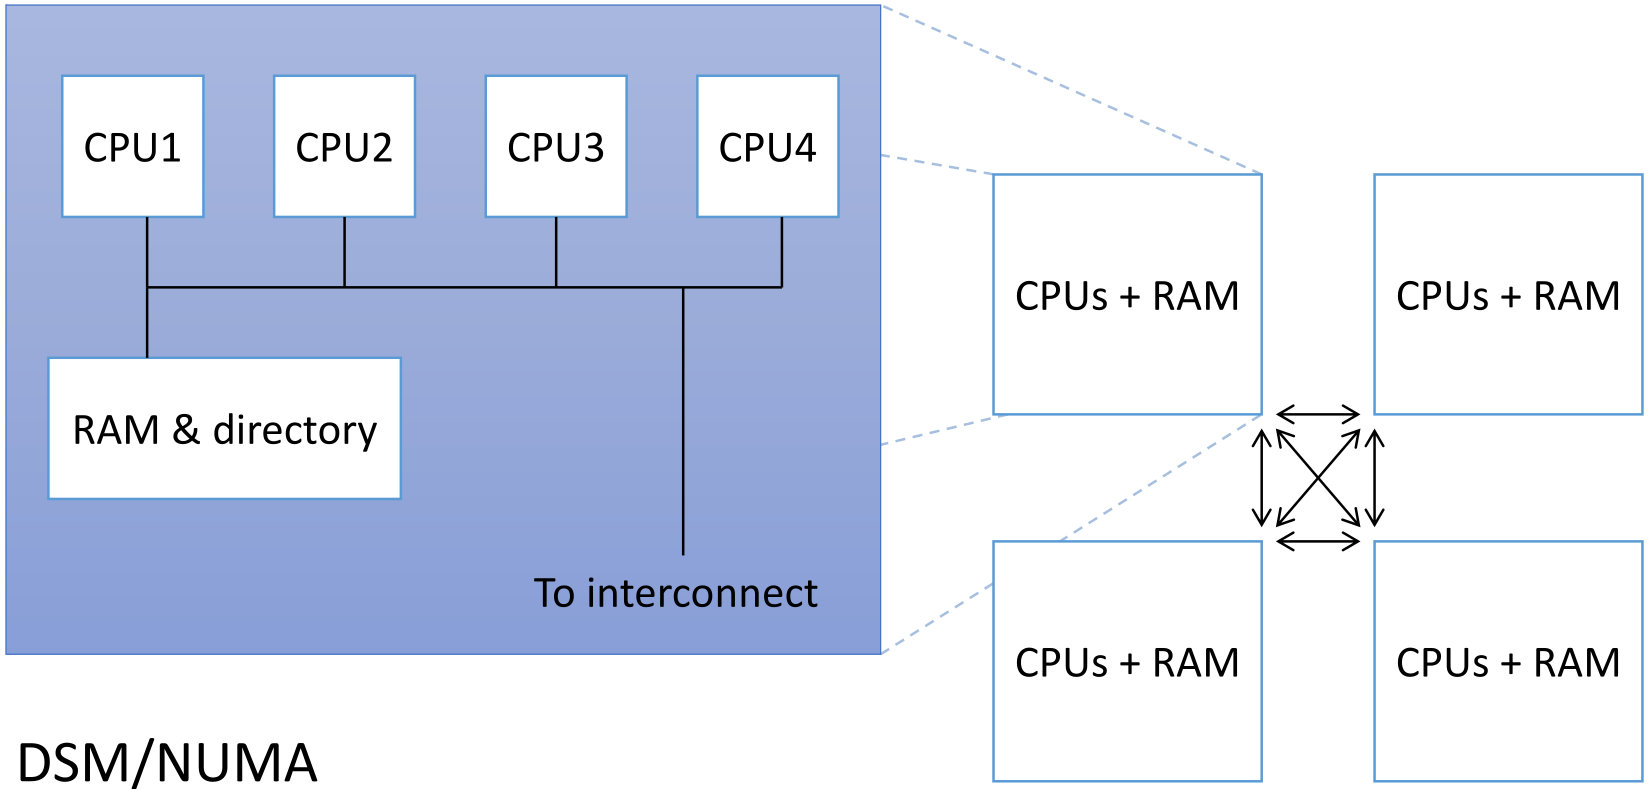
\includegraphics[width=0.8\textwidth]{24_DistributedMemoryArch.png}

\paragraph{Non-Uniform Memory Access}
Since the RAM each slice has is smaller than the main memory in SMP, access times to local memory faster. Access to RAM of other slices is possible to due to the shared address space (there is one single address space), but typically is much slower. The problem is how to figure out where certain data is and depending on its location, access takes non-uniform amount of time.

Another difficulty which arises from splitting cache is how to keep caches coherent.

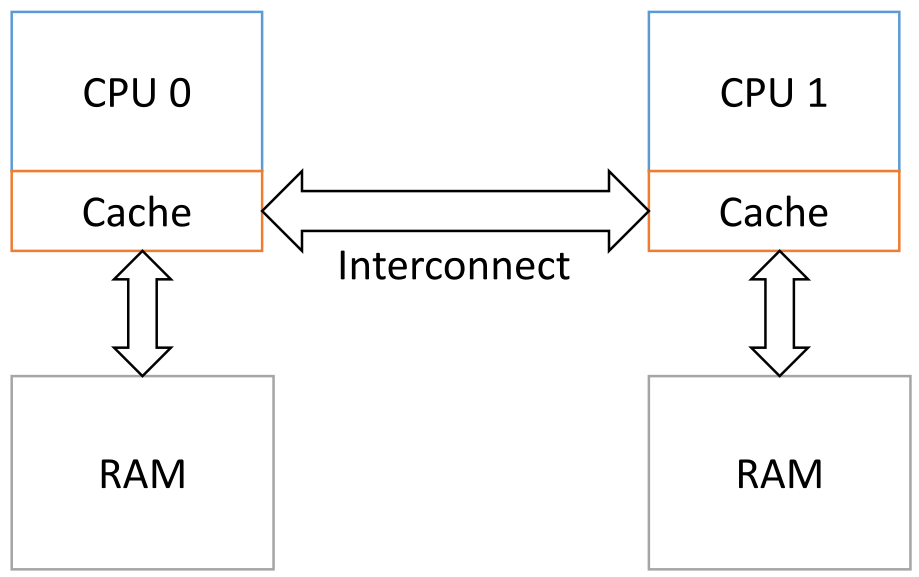
\includegraphics[width=0.8\textwidth]{24_MemoryAccess.png}

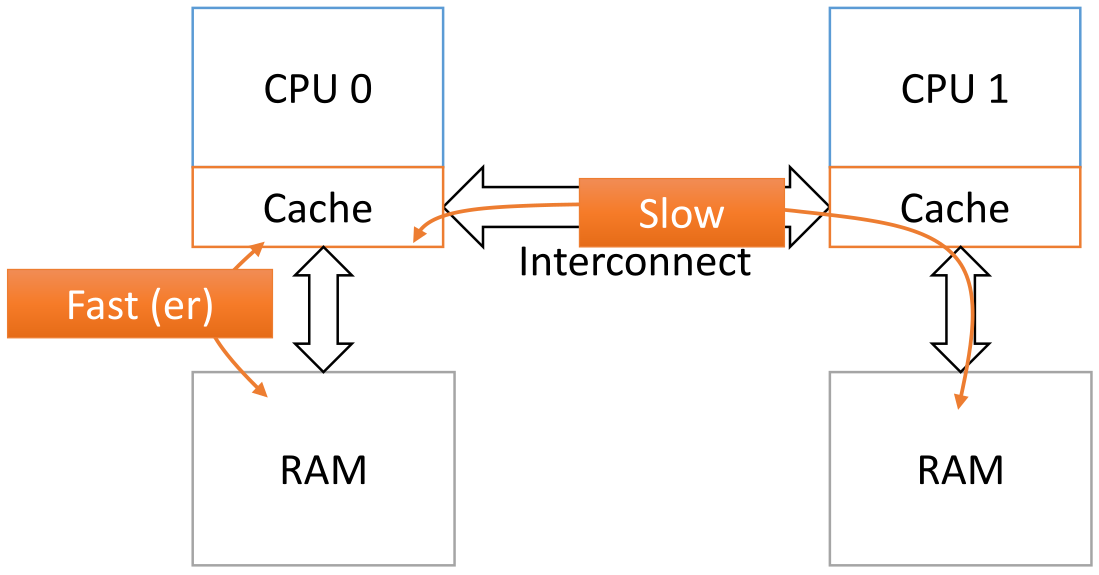
\includegraphics[width=0.8\textwidth]{24_MemoryAccessII.png}

\subsubsection{Cache Coherence}
CPUs cannot snoop anymore since there is no public bus. Possible solutions to overcome the resulting cache coherence problem are (we still want to be able to used the introduced cacher coherency protocols):

\paragraph{Bus emulation}
A shared bus is emulated, which allows CPUs to snoop again. In practice, this requires that each nodes sends a message to all other nodes and waits for a response from them before proceeding. This implementation is rather complex.

Simulate a bus, everyone sends messages to everyone else. 

\paragraph{Cache Directory}
For each cacheline we have some extra information. Together it is called cache directory. It stored the data itself, as well as things like who owns this data and which CPU node has this line currently. This way we do not need to broadcast messages related to this memory block to everyone but only the nodes which have a copy of this.

This method is useful when data is not widely shared among nodes and the when there are many NMUMA nodes. 

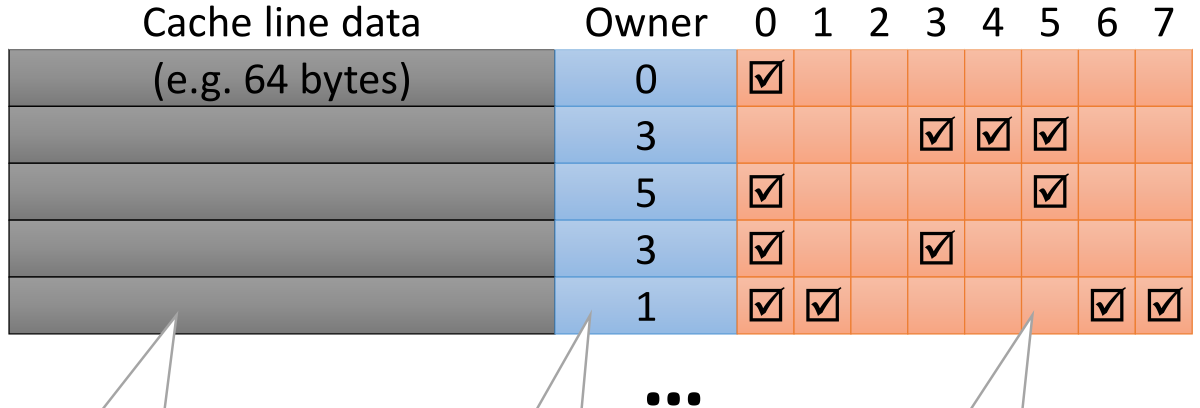
\includegraphics[width=0.8\textwidth]{24_CacheDirectory.png}

This is used in large multiprocessors.

\subsubsection{Performance Implications of Multicore}

\paragraph{Example: 8-Socket 32 Cores AMD Barcelona}
This architecture has a core local L1 and L2 cache, and a node shared L3 cache. Access of node local RAM or L3 is rather fast while access to other node's RAM or L3 gets slower the more hops we have to do. 

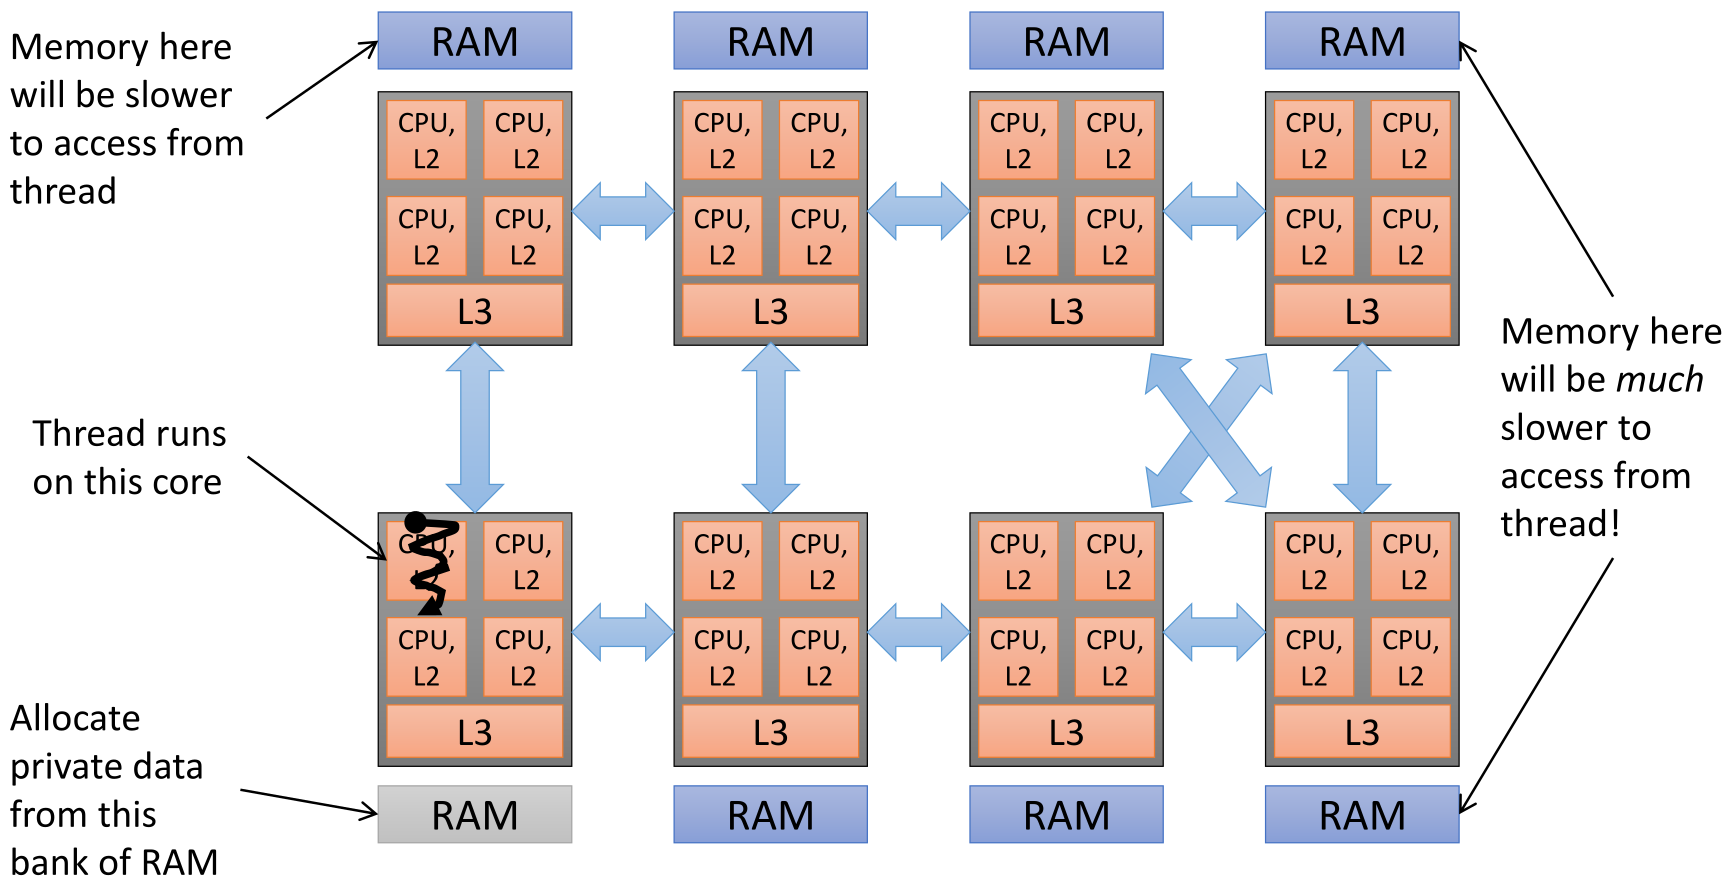
\includegraphics[width=0.8\textwidth]{24_MemoryLatency.png}


This typology is slightly unusual. It was split into two boards and the connection between the two boards is more expensive. Messages are not routed in the obvious way to make sure that not too many packages are sent at the time (or something like that). 

The left side has an additional PCI connection and therefore there is no crosslink. 

L3 is unified for the socket. All misses of the non-shared L2 goes to the L3. A line may be not in our L2 and not in our L3 but in someone else L2. That is a little weird but not unusual. 

\paragraph{False Sharing}
For a single CPU it is optimal when we have good locality, i.e. do many operations to the same cache line. But when there are multiple threads of different CPUs on different sockets which do that, we get a ping-pong effect between the caches on every write. This is very bad.

\subsubsection{Optimisation Example: MCS Locks}
There are many data structures which rely on locks. For NUMA architectures, cache lines containing a lock are a hot spot since many different thread on multiple sockets try to read and write it. This gets very expensive due to ping-pong of the cache line. The idea if MCS (acronym for Mellor-Crummey and Scott) is that threads spin on local data and only one processor wakes up and acquires the free lock.

This is possibly the best multiprocessors locking system which we have.

\paragraph{Implementation}
The idea is that we have a linked list. A thread which wants to acquire the lock adds itself to the linked list. Once the lock is released, the next CPU in the list is notified which then quires the lock.

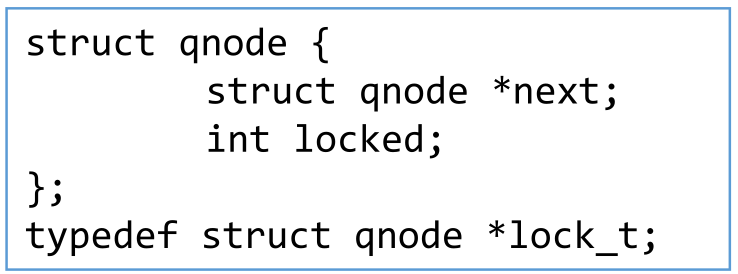
\includegraphics[width=0.8\textwidth]{24_ExQnode.png}

\subparagraph{Acquire}

\begin{enumerate}
    \item Add ourself to the end of the queue using \code{XCHG}.
    \item If the queue was empty we acquire the lock.
    \item If the queue was not empty, point previous tail to us and spin on local cache line.
\end{enumerate}

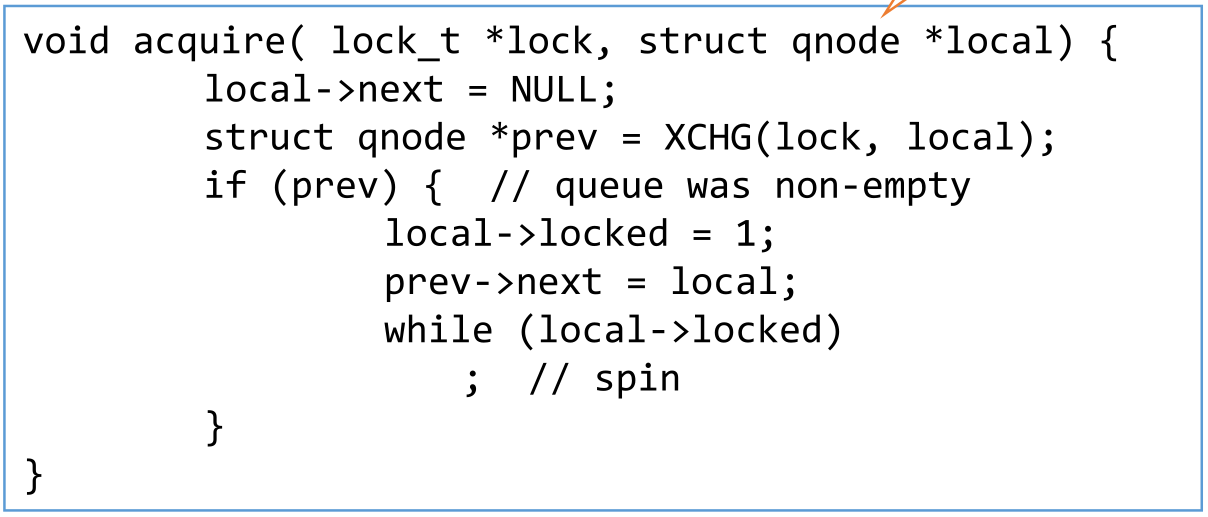
\includegraphics[width=0.8\textwidth]{24_ExAcquire.png}

The qnode, on which we spin is thread local.

\subparagraph{Release}
\begin{enumerate}
    \item We have the lock. Check is someone is waiting for the lock.
    \item If yes, we notify them and they will acquire the lock.
    \item If no, set the lock to \code{NULL} (unless someone appears in the meantime).
    \item If someone has appeared in the meantime, wait for them to enqueue and notify them.
\end{enumerate}

\paragraph{Spin Lock Comparison}
Spin lock to no scale well due to congestion, false sharing etc. 

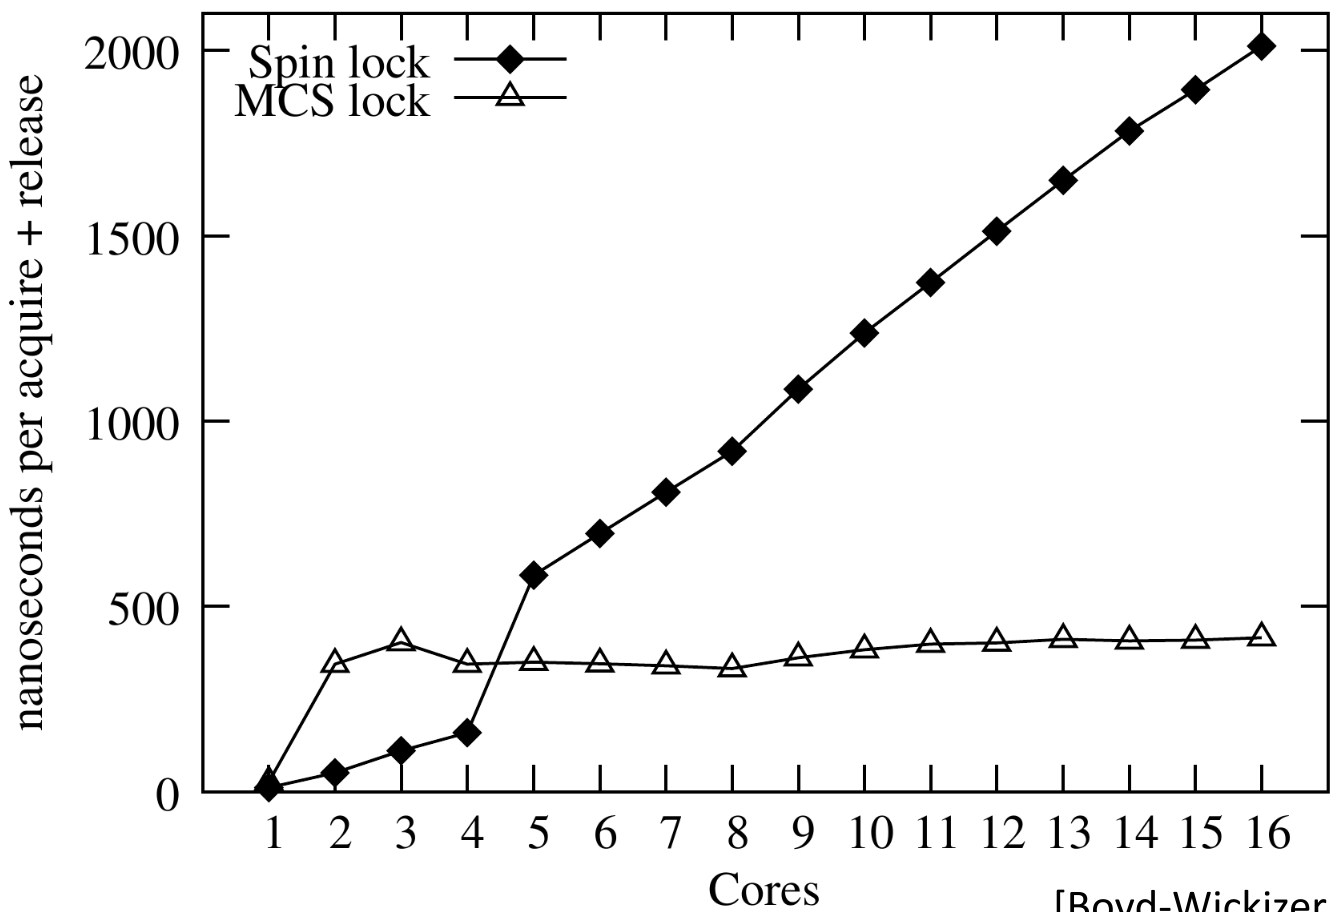
\includegraphics[width=0.8\textwidth]{24_LockPerformance.png}

\subsection*{Devices}
Devices are hardware which interact with the OS through some kind of software. They are connected via a bus (e.g. PCI) and we communicate with them via a set of shared registers (CPU and device can read/write). Devices can cause interrupts and data can be transfered to/from them using \textit{Direct Memory Access} without work from the CPU.

\subsubsection{Device Registers}
CPUs can read device registers for:

\begin{itemize}
    \item Obtaining status information
    \item Read input data
\end{itemize}

CPUs can write to device registers for:
\begin{itemize}
    \item Set device into a certain state and reset the state
    \item Configure the device in a certain way
    \item Write output data
\end{itemize}

Device registers are conceptually different from CPU registers. They can be addressed in two ways. Both are supported by x86.

\paragraph{Memory Mapped}
When the device registers are memory mapped, they appear to the system as a memory location and hence, common operations like loads and stores can be used in them. This is a great advantage and allows for much more flexibility compared to the second approach.

Device drivers are responsible for correctly initializing the device.

This is the most commonly used approach today.

\paragraph{I/O Instructions}
There are separated, dedicated instructions to communicate with the device. There is also a separate address space, the I/O address space. This space is typically smaller, e.g. $16$ bits.

\paragraph{Summary}
Both of the introduced methods are used today.

Device registers behave differently from regular RAM. But device registers are actually volatile (change without warning). They are not meant to save data but used for communication. RAM only changes when the CPU changes it but device registers are also manipulated by the device. When writing to a device register we also expect to trigger a certain action. Cs volatile instruction is useful to use in conjunction with device registers to mark to the CPU do not e.g. optimise away such instructions.

\paragraph{Example: National Semiconductor ns16550 UART}
UART used to be a very common and was used for serial communication. It is connected to the south bridge.

South bridge is for IO while the north bridge is for CPU.

This device is pretty much the standard even though it is not heavily used anymore.

Datasheets about the device are used to figure out how to interact with a device. Often they are rather poorly written and not very accurate.

UART has for example the following registers, each of then is $8$ bit long.

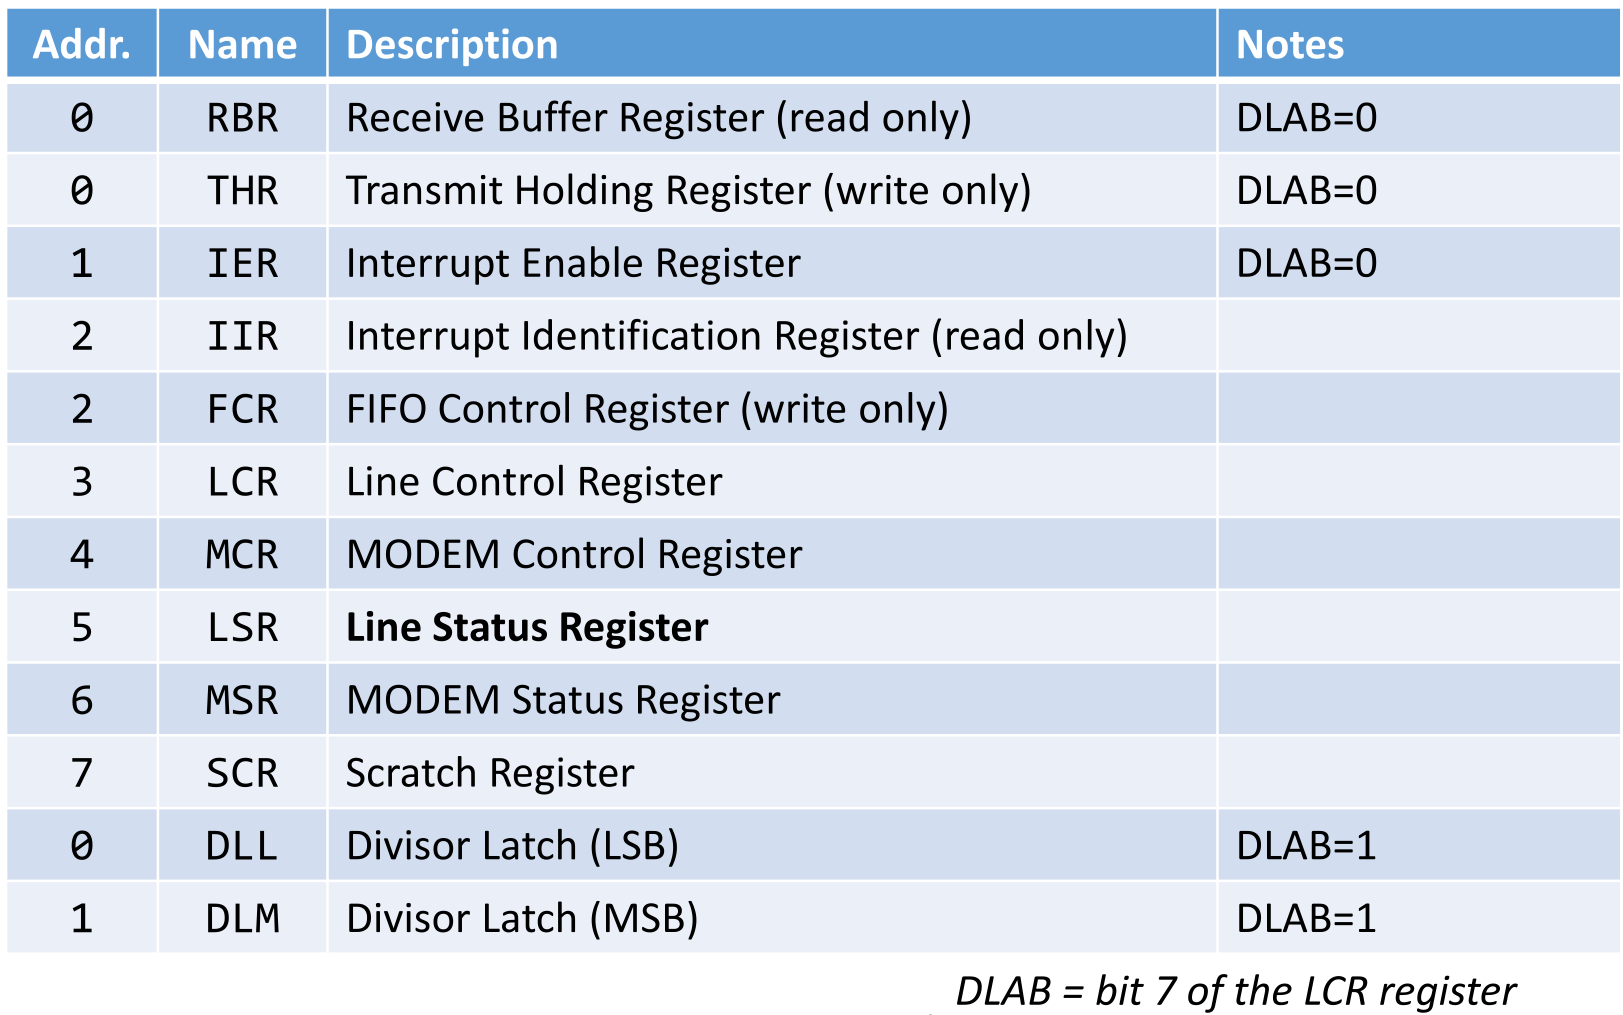
\includegraphics[width=0.8\textwidth]{24_UartRegister.png}

The DLAB bit is devicor latch access bit and is part of the LSR. Depending on this bit, the purpose of certain registers differ.

The address starts at $0$ but that is just the offset from the memory mapped IO base address.

In the Line Status Registers, different bits have different meaning.

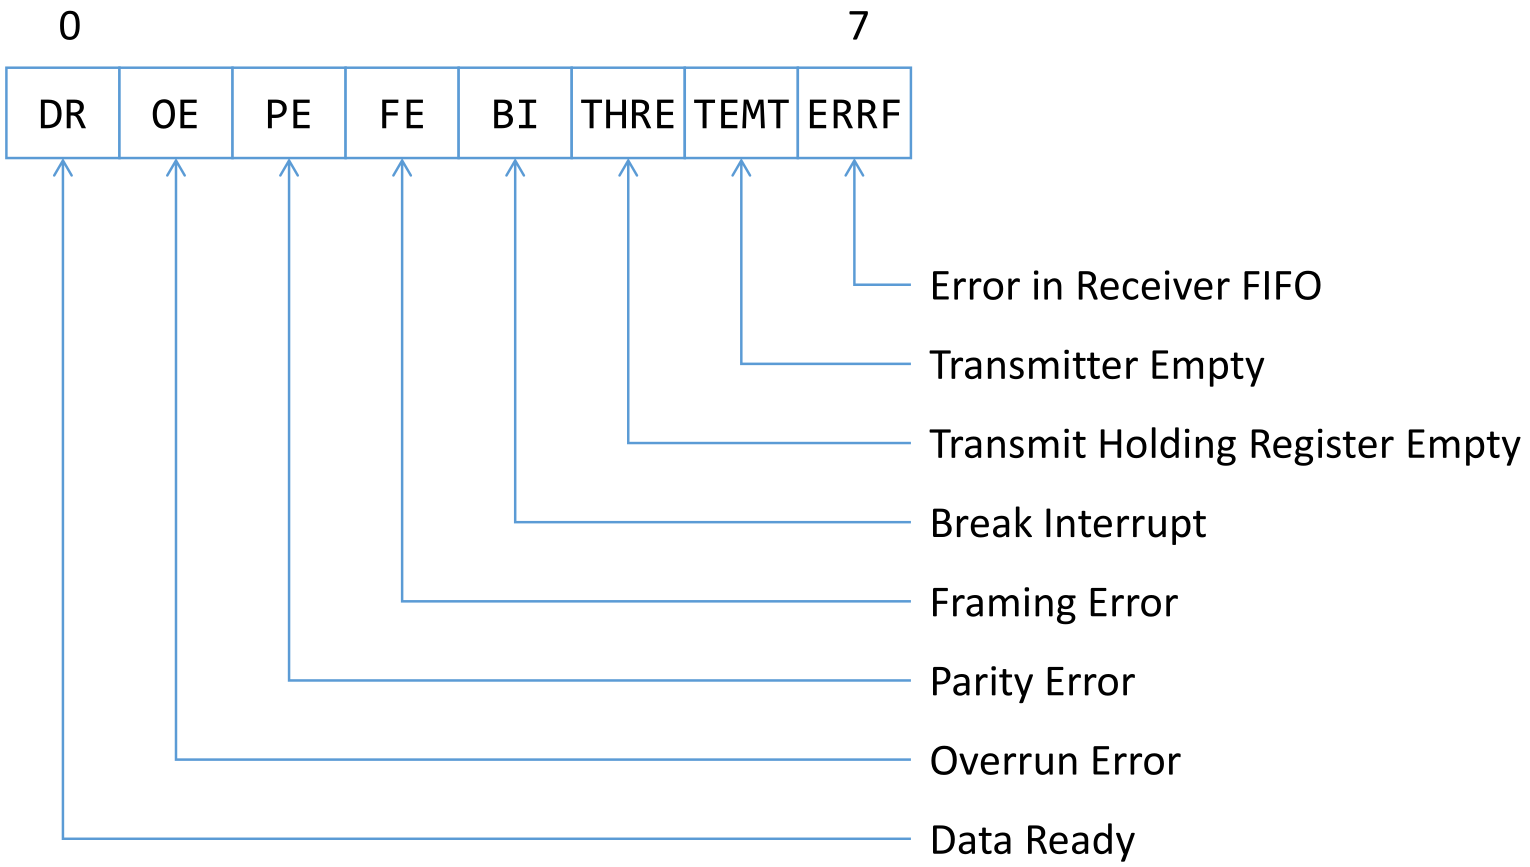
\includegraphics[width=0.8\textwidth]{24_UartLineStatusRegister.png}

\subparagraph{Simple UART Driver}
The following is a very simplified UART driver, containing no initialisation, no error handling etc.

At first we define the base register of the device register. This information is taken from the datasheet.

For sending a character, we first have to make sure that we can actually write a new char to the device by bitmasking the right register. We spin loop fill we are successful and when this is the case, we write our character to a designated device register. To read, we do again spin loop and check the ready bit if there is data to be read. When there is, we read the data from the register.

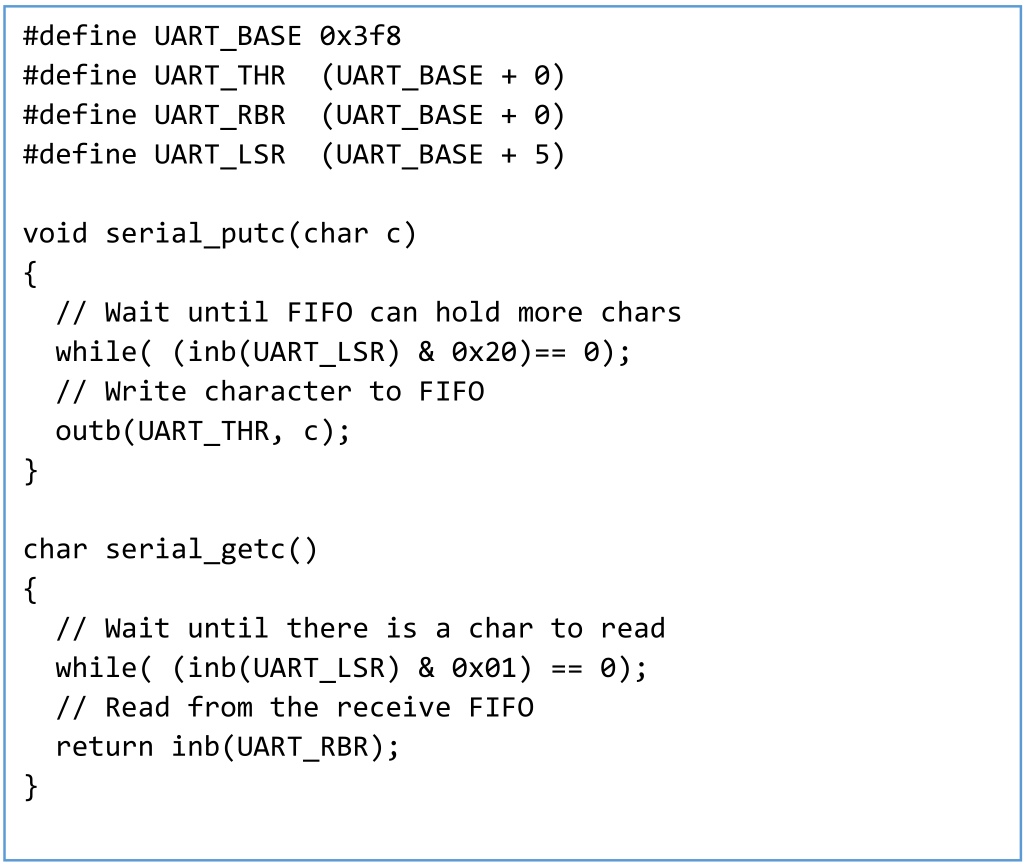
\includegraphics[width=0.8\textwidth]{24_UartDriver.png}

\paragraph{Summary}
The simple driver uses \textit{Programmed I/O (PIO)} (which is in contrast to \textit{Direct Memory Accessed}). This means that the CPU does explicitly read/write values from registers and hence, all data passes through the CPU.

Also, the simple drives uses polling to wait for a certain condition. An alternative would be to use interrupts, where we are notified, when a certain condition is reached. In polling $100\%$ CPU is used just for waiting. But its advantage is that that it can take action as soon as a condition is reached (there is not need to wait for a notification). Interrupts are superior when there is very infrequent arrival of information.

Drivers are part of the OS. Device drivers are a significant portion of the code (about $70\%$).

\subsubsection{Dealing with Caches}
We cannot use caching for device registers since these registers are volatile (the device can change the registers too). This would lead to inconsistent caches.

Write-back caches and write buffers are also problematic because changes are not visible to the device immediately.

Also, read and writes cannot be combined into cache lines (not sure that they meant by that).

As a consequence, device registers must bypass cache. In the page table there was a flag to indicate that a certain page should not be cached. They are used for this purpose.
